% Created 2025-03-25 Tue 12:30
% Intended LaTeX compiler: pdflatex
\documentclass[conference]{IEEEtran}
\usepackage[utf8]{inputenc}
\usepackage[T1]{fontenc}
\usepackage{graphicx}
\usepackage{longtable}
\usepackage{wrapfig}
\usepackage{rotating}
\usepackage[normalem]{ulem}
\usepackage{amsmath}
\usepackage{amssymb}
\usepackage{capt-of}
\usepackage{hyperref}
\IEEEoverridecommandlockouts
\usepackage{cite}
\usepackage{amsmath,amssymb,amsfonts}
\usepackage{algorithmic}
\usepackage{graphicx}
\usepackage{textcomp}
\usepackage{xcolor}
\usepackage[hidelinks]{hyperref}
\usepackage{hanging} %% for IEEE-style hanging indent in References section.
\input{/home/praaneshnair/.config/doom/def.tex}
\input{/home/praaneshnair/.config/doom/author.tex}
\graphicspath{ {.} }
\date{}
\title{Prediction of Ground Motion using Data on Seismic Waves}
\hypersetup{
 pdfauthor={Praanesh Balakrishnan Nair},
 pdftitle={Prediction of Ground Motion using Data on Seismic Waves},
 pdfkeywords={},
 pdfsubject={},
 pdfcreator={Emacs 29.4 (Org mode 9.7.19)}, 
 pdflang={English}}
\begin{document}

\maketitle
\begin{abstract}
This paper presents a methodology for analyzing seismic data from significant
earthquakes using the ObsPy Python library. Our dataset encompasses four major
seismic events: the 2011 Tohoku earthquake (Japan), the 2010 Chile earthquake,
the 2016 Kumamoto earthquake (Japan), and the 2015 Nepal earthquake. The utility
of the processed data is demonstrated by applying the Short-Term
Average/Long-Term Average (STA/LTA) algorithm to the mean-subtracted waveforms
to automatically identify the arrival of P-Waves and S-Waves. A k-Nearest
Neighbours (kNN) regression model was used to predict the peak ground
acceleration (PGA) and Arias intensity for each event.


\end{abstract}


\begin{IEEEkeywords}

Seismic Waves, Instrument Response, Ground Acceleration, Arias Intensity

\end{IEEEkeywords}
\section{Introduction}
\label{sec:orga2d6b84}
The analysis of seismic data provides crucial insights into earthquake dynamics
and Earth's subsurface structure. Various seismic waveform data from several
significant earthquakes were processed and analyzed by investigating the
relationship between maximum amplitude and distance to the event. This was done
by extracting features, using matrix operations and similarity measures. We
focus on four major seismic events: the 2011 Tohoku earthquake (Japan), the 2010
Chile earthquake, the 2016 Kumamoto earthquake (Japan), and the 2015 Nepal
earthquake. This approach facilitates access to a large volume of data from
diverse sources.
\section{Methodology}
\label{sec:orgd0acd6f}
\subsection{Data Preprocessing}
\label{sec:orgdd4851c}
The ObsPy Python library was used for obtaining seismic wave data withint 20
degrees of the epicenter. Using \texttt{obspy.mass\_downloader()}, waveform data
was retrieved in miniSEED format corresponding station metadata in StationXML
format from multiple data centers, including IRIS. The downloaded miniSEED files
were processed to extract key features for analysis. Time-domain data was
converted into CSV files and statistical measures such as mean, standard
deviation, maximum amplitude, peak-to-peak amplitude, root mean square, dominant
frequency, spectral centroid and energy were added to it. Crucially, station
metadata, including station ID, channel, start time, latitude, longitude,
elevation, and distance from the event, were also incorporated into the CSV
files. This enriched dataset allows for comprehensive analysis, linking waveform
characteristics with station location and event information.

The data was categorized into three classes based on the maximum amplitude: the
first 33rd percentile was assigned to class 0, the next 33rd percentile to class
1, and the remaining data to class 2. For these classes, the mean (class
centroid) and standard deviation (class spread) of the data points were
calculated.
\subsection{Training}
\label{sec:orgb267510}
We trained a weighted k-Nearest Neighbors (k-NN) classifier to predict the class
labels based on maximum amplitude and distance. Peak ground acceleration was
predicted using several features such as the distance from the station to the
earthquake epicenter (in degrees), geographical coordinates of the station, the
elevation of the station, the frequencies with the most energy in the signal and
the weighted average frequency in the signal. The k-NN model predicts peak
ground acceleration at new locations by finding the 5 most similar locations in
the feature space and averaging their values of peak ground acceleration,
weighted by distance.

80\% of the data was used for training and 20\% for testing. We further explored
the impact of the hyperparameter k by training and testing models with k values
ranging from 1 to 11, observing the resulting accuracy trends.
\section{Results}
\label{sec:orga8e12bd}
A plot between the maximum amplitude against distance to the event, and a
histogram of maximum amplitudes were generated. We evaluated the
performance of the k-NN classifier with k = 3, achieving a high accuracy of
0.99. The k=3 model demonstrated a training accuracy of 1.00 and a testing
accuracy of 0.99, indicating neither underfitting nor overfitting.

\begin{figure}[htbp]
    \centering
    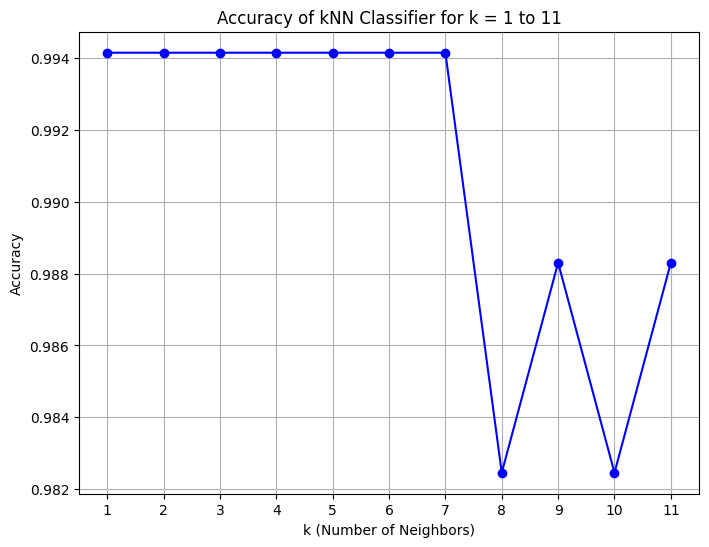
\includegraphics[width=\columnwidth]{knn_accuracy.png}
    \caption{Accuracy of k-NN Classifiers with Different Values of 'k'}
    \label{fig:example}
\end{figure}


\begin{figure}[htbp]
    \centering
    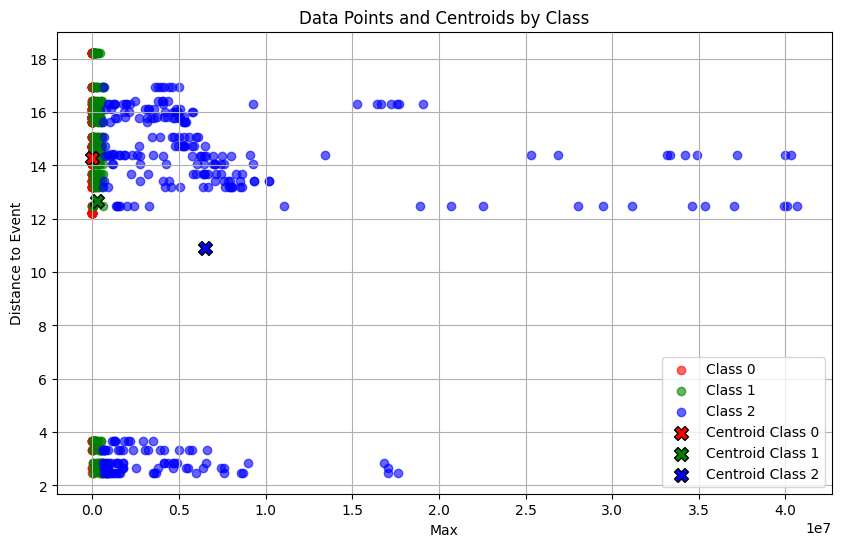
\includegraphics[width=\columnwidth]{datapoints_and_centroids_by_class.png}
    \caption{Data Points and Centroids by Class}
    \label{fig:example}
\end{figure}

The Euclidean distances between the class centroids showed indication of highly
distinguishable classes. The distance are shown below.

\begin{table}[htbp]
\caption{Euclidean Distances}
\centering
\begin{tabular}{lr}
Classes Taken & Distance\\
\hline
0 and 1 & 262577.78\\
0 and 2 & 262577.78\\
1 and 2 & 6228234.60\\
\end{tabular}
\end{table}


The Minkowski distance between class centroids was calculated for orders from 1
to 10.

\begin{figure}[htbp]
    \centering
    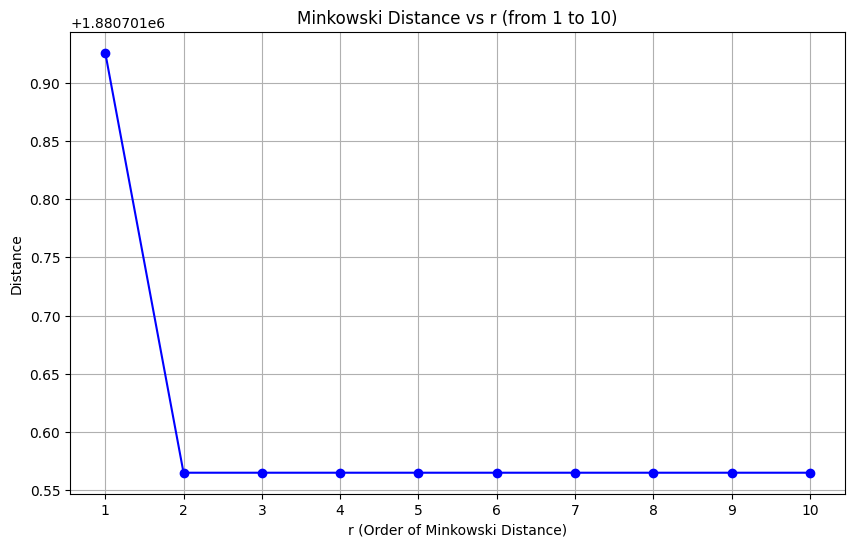
\includegraphics[width=\columnwidth]{minkowski_distance.png}
    \caption{Minkowski Distances of Different Orders}
    \label{fig:example}
\end{figure}

The below table demonstrates the performance metrics on training.

\begin{table}[htbp]
\caption{Training Classification Report}
\centering
\begin{tabular}{lrrrr}
 & precision & recall & f1-score & support\\
\hline
1 & 1.00 & 1.00 & 1.00 & 200\\
2 & 1.00 & 1.00 & 1.00 & 197\\
accuracy &  &  & 1.00 & 397\\
macro avg & 1.00 & 1.00 & 1.00 & 397\\
weighted avg & 1.00 & 1.00 & 1.00 & 397\\
\end{tabular}
\end{table}

On testing the data, the performance metrics were obtained as demonstrated in the below table.

\begin{table}[htbp]
\caption{Test Classification Report}
\centering
\begin{tabular}{lrrrr}
 & precision & recall & f1-score & support\\
\hline
1 & 0.97 & 1.00 & 0.99 & 80\\
2 & 1.00 & 0.99 & 0.99 & 91\\
accuracy &  &  & 0.99 & 171\\
macro avg & 0.99 & 0.99 & 0.99 & 171\\
weighted avg & 0.99 & 0.99 & 0.99 & 171\\
\end{tabular}
\end{table}

The training confusion matrix is shown below.
\begin{equation}
\begin{bmatrix}
200 & 0 \\
0 & 197
\end{bmatrix}
\end{equation}


The testing confusion matrix is shown below.

\begin{equation}
\begin{bmatrix}
80 & 0 \\
1 & 90
\end{bmatrix}
\end{equation}
\section{Literature Survey}
\label{sec:org5aae6e6}
Seismic signal processing and analysis have garnered significant attention in
recent years, with various machine learning methodologies being employed for
classification, event detection, and predictive modeling. This section reviews
key contributions in the field, highlighting different approaches and techniques
applied to seismic data analysis.


Li et al. \cite{b1} investigated seismic data
classification using supervised machine learning techniques. Their study focused
on extracting features such as spectral content, amplitude variations, and
waveform characteristics. They evaluated the performance of multiple machine
learning models, including Support Vector Machines (SVM), Decision Trees, and
Neural Networks, which were trained on labeled seismic event datasets to assess
classification accuracy.


Ramirez and Meyer \cite{b2} explored seismic phase
classification through manifold learning techniques. Their approach involved
mapping high-dimensional seismic data onto a lower-dimensional manifold using
Laplacian Eigenmaps, improving classification performance by preserving local
waveform structures. Their method demonstrated enhanced differentiation between
P-waves and S-waves using nearest-neighbor-based classifiers in the transformed
space.


Chakraborty et al. \cite{b3} employed statistical feature extraction
techniques for micro-seismic event detection. The extracted features included
peak amplitude, energy, zero-crossing rate, and entropy. Machine learning models
such as Random Forest, SVM, and k-Nearest Neighbors (KNN) were applied to
classify seismic events, distinguishing natural seismic activity from noise with
improved accuracy.


Shu et al. \cite{b4} conducted a comprehensive survey on
machine learning applications in microseismic signal recognition and
classification. They categorized methodologies into three major groups:
feature-based models utilizing statistical descriptors, deep learning models
such as Convolutional Neural Networks (CNNs) and Recurrent Neural Networks
(RNNs), and hybrid techniques that integrate statistical feature extraction with
deep learning frameworks. Additionally, their survey highlighted key challenges
and potential advancements in the domain.


Varshney et al. \cite{b5} developed a
machine learning-based earthquake monitoring system leveraging real-time seismic
data streams. Their approach involved preprocessing seismic data using Fourier
and Wavelet Transforms before training classification models, such as Decision
Trees and Neural Networks, to detect and monitor earthquake events dynamically.


Chin et al. \cite{b6} enhanced earthquake detection accuracy by implementing a
hybrid deep learning model integrating CNNs and Long Short-Term Memory (LSTM)
networks. Their framework, trained on labeled seismic waveform datasets,
incorporated data augmentation techniques to improve model robustness. The
proposed system demonstrated superior detection performance compared to
traditional signal processing methods.


Shimshoni and Intrator \cite{b7} applied
ensemble learning techniques for seismic signal classification. Their work
utilized bagging and boosting strategies to enhance classification accuracy,
demonstrating that ensemble-based neural network approaches could improve
differentiation between seismic events.


Agliz and Atmani \cite{b8} employed
multi-layer perceptron (MLP) neural networks for seismic signal classification.
Their methodology involved extracting both frequency-domain and time-domain
features from seismic waveforms, which were subsequently used as input to the
neural network for classification and training.


Akhouayri et al. \cite{b9}
introduced a fuzzy expert system for automatic seismic signal classification.
Their method defined fuzzy sets based on key signal parameters such as
amplitude, frequency content, and duration, allowing for a more flexible and
interpretable classification framework compared to traditional rule-based
systems.


Curilem et al. \cite{b10} investigated the application of genetic
algorithms for optimizing neural network classifiers in the context of volcanic
seismic signal classification. Their findings demonstrated that evolutionary
computation techniques could enhance the performance of neural network models in
differentiating between various types of volcanic seismic events.



\begin{thebibliography}{00}
\bibitem{b1} W. Li, N. Narvekar, N. Nakshatra, N. Raut, B. Sirkeci and J. Gao, ``Seismic Data Classification Using Machine Learning,'' \textit{2018 IEEE Fourth International Conference on Big Data Computing Service and Applications (BigDataService)}, Bamberg, Germany, 2018, pp. 56-63
\bibitem{b2} J. Ramirez Jr and F. G. Meyer, ``Machine Learning for Seismic Signal Processing: Phase Classification on a Manifold,'' \textit{2011 10th International Conference on Machine Learning and Applications and Workshops}, Honolulu, HI, USA, 2011, pp. 382-388
\bibitem{b3} M. Chakraborty, M. Das and S. Aruchamy, ``Micro-Seismic Event Detection using statistical feature extraction and machine learning techniques,'' 2\textit{022 IEEE 7th International conference for Convergence in Technology (I2CT)}, Mumbai, India, 2022, pp. 1-5
\bibitem{b4} H. Shu, A. Y. Dawod, L. Mu and W. Tepsan, ``A Survey of Machine Learning Applications in Microseismic Signal Recognition and Classification,'' \textit{2023 15th International Conference on Software, Knowledge, Information Management and Applications (SKIMA)}, Kuala Lumpur, Malaysia, 2023, pp. 18-23
\bibitem{b5} N. Varshney, G. Kumar, A. Kumar, S. K. Pandey, T. Singh and K. U. Singh, ``Machine Learning Based Algorithm for Earthquake Monitoring,'' \textit{2023 IEEE 12th International Conference on Communication Systems and Network Technologies (CSNT)}, Bhopal, India, 2023, pp. 264-270
\bibitem{b6} T. -L. Chin, C. -Y. Huang, S. -H. Shen, Y. -C. Tsai, Y. H. Hu and Y. -M. Wu, ``Learn to Detect: Improving the Accuracy of Earthquake Detection,'' in \textit{IEEE Transactions on Geoscience and Remote Sensing}, vol. 57, no. 11, pp. 8867-8878, Nov. 2019
\bibitem{b7}Y. Shimshoni and N. Intrator, ``Classification of seismic signals by integrating ensembles of neural networks,'' in \textit{IEEE Transactions on Signal Processing}, vol. 46, no. 5, pp. 1194-1201, May 1998
\bibitem{b8}Agliz, Driss, and Abderrahman Atmani. ``Seismic signal classification using multi-layer perceptron neural network.'' \textit{International Journal of Computer Applications} 79, no. 15 (2013).
\bibitem{b9}Akhouayri, Es-Saïd, Dris Agliz, Daniele Zonta, and Abderrahman Atmani. ``A fuzzy expert system for automatic seismic signal classification.'' \textit{Expert Systems with Applications} 42, no. 3 (2015): 1013-1027.
\bibitem{b10}Curilem, Gloria, Jorge Vergara, Gustavo Fuentealba, Gonzalo Acuña, and Max Chacón. ``Classification of seismic signals at Villarrica volcano (Chile) using neural networks and genetic algorithms.'' \textit{Journal of volcanology and geothermal research} 180, no. 1 (2009): 1-8.
\end{thebibliography}
\end{document}
